\documentclass[../main.tex]{subfiles}
\begin{document}

\chapter{Emission processes in AGN}
\label{cap:emission}

AGN emission spans over the complete electromagnetic spectra, starting from the lowest observable radio frequencies to the highest energies of the $\gamma$-rays.
Several processes, divided among continuum processes such as synchrotron emission, thermal emission, inverse Compton emission, and atomic and molecular transitions, both permitted and forbidden, contribute to this ultra wide band emission.
In this chapter I will describe the main processes characterizing AGN emission in the radio and optical bands.

\section{Synchrotron emission}
\label{sec:synchrotron}

\blfootnote{This section is partially extracted from \citet{Beckmann12}.}
Synchrotron emission is one of the main mechanism of continuum emission in AGN, especially in radio-loud ones.
It is classified as a non-thermal process, because the particle involved in the process usually are not in thermodynamical equilibrium.
Synchrotron emission is the dominant emission mechanism in the radio region of an AGN broad band spectrum, also called spectral energy distribution (SED), but it can be responsible of a significant amount of emission up to optical and UV wavelengths, especially in peculiar classes of AGN such as blazars.
Synchrotron emission occurs when charged particles, usually electrons, are accelerated in a magnetic field.
If the electron has a velocity component perpendicular to the magnetic field, it starts spiraling because of the Lorentz force.
The energy emitted by a single electron is a function of its energy, of the magnetic field strength $B$ and of the angle between the field and the direction of motion of the particle.

To calculate the spectrum emitted by a population of electrons it is possible to start considering a single electron with charge $e$, rest mass $m$ and Lorentz factor:

\begin{equation}
    \label{eq:lorentz}
    \gamma = \frac{1}{\sqrt{1-\frac{v^2}{c^2}}}.
\end{equation}

The electron is traveling with velocity $\vec{v}$ through a uniform and static magnetic field $\vec{B}$.
The force acting on the electron is:

\begin{equation}
    \label{eq:mag_force}
    \frac{d}{dt}(\gamma m \vec{v})=\frac{e}{c}\left(\vec{v}\times\vec{B}\right),
\end{equation}
and, because of the cross product, it is always perpendicular to the motion of the particle.
This means that the magnitude of its velocity $v$ and the Lorentz factor $\gamma$ are constant.
The force is also perpendicular to the direction of the magnetic field, which implies that $v_{\parallel}$, and consequently $v_{\bot}$ ($v^2 = v^2_{\parallel} + v^2_{\bot}$), is constant.
The final result is that the electron motion will be a combination of a circular motion with constant radius $r_g$ around the magnetic field lines and a motion at constant velocity ($v_{\parallel}$) along the field lines.
The radius $r_g$ is called gyroradius and it is defined as:

\begin{equation}
    \label{eq:gyroradius}
    r_g = \frac{v_{\bot}\gamma m c}{e B}.
\end{equation}
From the gyroradius it is possible to define the frequency of the circular motion, the Larmor frequency:
\begin{equation}
    \label{eq:larmor_freq}
    \nu_g = \frac{e B}{2\pi \gamma m c},
\end{equation}
and the angular gyrofrequency $\omega_g = 2\pi \nu_g$.
The total luminosity produced by the acceleration process can be derived from the following equation \citep{Rybicki86}:

\begin{equation}
    \label{eq:rybicki}
    L = \frac{2e^2}{3c^3}\gamma^4\left[\left(\frac{d\vec{v_{\bot}}}{dt}\right)^2+\gamma^2\left(\frac{d\vec{v_{\parallel}}}{dt}\right)^2\right],
\end{equation}
considering that $d\vec{v_{\parallel}}/dt = 0$, the acceleration is perpendicular to the velocity, and that $d\vec{v_{\bot}}/dt = \omega_g\vec{v_{\bot}}$, because the electron follows a circular motion.
Since $v_{\bot} = v\sin\beta$, where $\beta$ is the pitch angle, $v$ is the magnitude of its velocity, and assuming an isotropic distribution of particle velocities during the integration over the angles, the final synchrotron luminosity is:
\begin{equation}
    \label{eq:sync_lum}
    L  = \frac{4e^4B^2\gamma^2v^2}{9c^5m^2}.
\end{equation}

This formula has been derived considering the case of an electron. 
However, it can be used also to describe the synchrotron emission of a positron, same mass but different sign of the charge, or of a proton, different mass and different charge sign.
However it is clear that since $L\propto m^{-2}$ the lighter is the emitting particle, the more luminous is the emission if the particle velocity is the same in all cases.
Since $m_p \sim 1836\cdot m_e$, the emission of a proton would be a factor $\sim 10^{-7}$ lower with respect to the emission of an electron (or positron) moving at the same speed, and so the latter is by far a more efficient emitter.
This consideration is important when discussing the nature of the particles producing synchrotron emission in relativistic jets.
To produce the same luminosity a jet made of proton should be significantly faster than a jet of electrons or positrons, which is the reason why electron powered jets seem more plausible.

If only the case of electron or positrons is considered, the formula can be simplified further:

\begin{equation}
    \label{eq:sync_semp}
    L=\frac{4}{3}\sigma_t\frac{v^2}{c}\gamma^2U_B,
\end{equation}

where $U_B = B^2/8\pi$ is the magnetic energy density and $\sigma_t$ is the Thomson cross-section:

\begin{equation}
    \label{eq:thomson}
    \sigma_t = \frac{8\pi}{3}\left(\frac{e^2}{mc^2}\right)^2.
\end{equation}

If the electron is highly relativistic ($v\sim c$) the synchrotron luminosity is a function only of the Lorentz factor and of the magnetic energy density.

An important property of the synchrotron radiation is that it is not emitted isotropically.
Because of relativistic beaming effects the radiation is concentrated in a narrow cone pointed towards the motion of the particle (Fig.\,\ref{fig:synchrotron}).
The opening angle of the cone $\phi$ is a function of the $\gamma$ factor of the particle, in particular $\phi \propto \gamma^{-1}$.
This produces a lighthouse effect and the observer will detect radiation only when the cone is pointing towards the line of sight.
The emission will be a short pulse of duration $\Delta t \sim 0.5\gamma^{-2} \omega_g^{-1}$, and the observed frequency will then be:
\begin{equation}
    \label{eq:new_freq}
    \nu \sim \Delta t^{-1} \sim \gamma^2\nu_g = \frac{\gamma^3v}{2\pi r_0},
\end{equation}
where $r_0$ is the gyroradius in the non-relativistic approximation ($\gamma \sim 1$).
If the radiation emitted by the electron is averaged over the entire rotation it will appear concentrated in a solid angle pointed towards the direction of the motion parallel to the magnetic field.

\begin{figure}
\centering
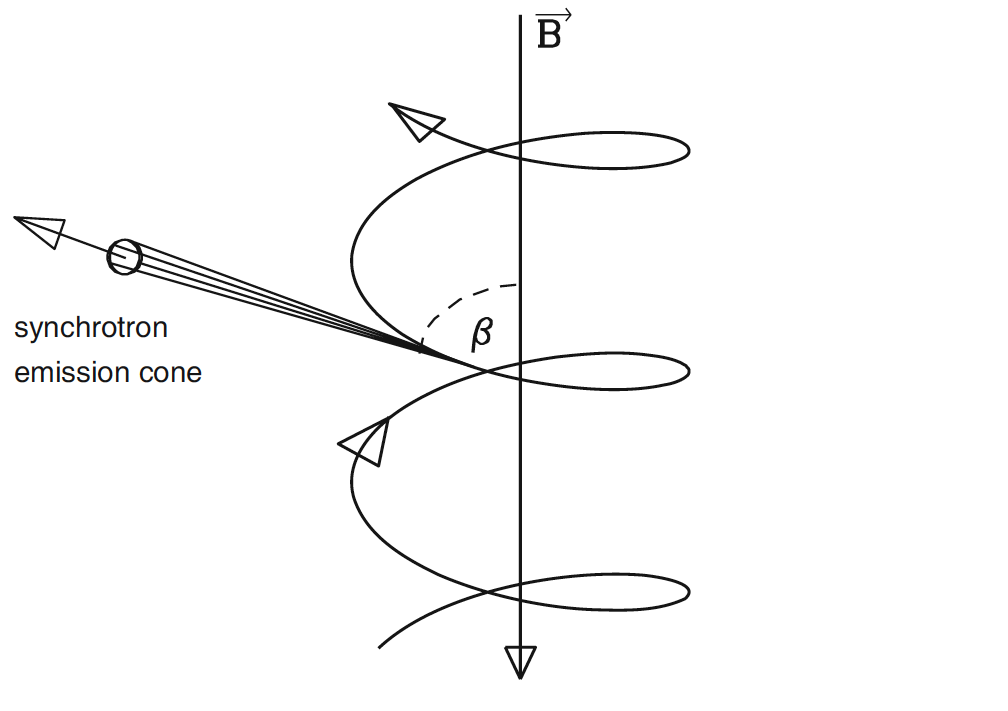
\includegraphics[width=0.8\textwidth]{images/synchrotron.png} 
\caption[]{Scheme of synchrotron emission by a relativistic electron with pitch angle $\beta$ from \citet{Beckmann12}. The emission is beamed in the direction of motion and forms a cone with opening angle $\phi\sim\gamma^{-1}$. If the emission is averaged over the entire rotation, it will be concentrated inside a solid angle pointing in the forward direction (top of the figure). }
\label{fig:synchrotron}
\end{figure}

The effective synchrotron spectrum emitted by an electron requires complex calculations to be derived \citep{Rybicki86}, but it is found that, averaging over the orbit, it is a continuum spectrum strongly peaked at the frequency $0.29\nu_c$ where $\nu_c $ is the critical frequency:

\begin{equation}
    \label{eq:critical_freq}
    \nu_c = \frac{3}{2} \gamma^3 \nu_g \sin \beta.
\end{equation}
The power per unit frequency of the spectrum is given by:
\begin{equation}
    \label{eq:shape}
    L(E,\nu) = \frac{\sqrt{3}e\gamma^2B\sin\beta}{m c^2}\frac{nu}{\nu_c}\int_{\nu/\nu_c}^\infty K_{5/3}(\xi)d\xi,
\end{equation}
where $K_{5/3}$ is the modified Bessel function of order $5/3$.

\begin{figure}
\centering
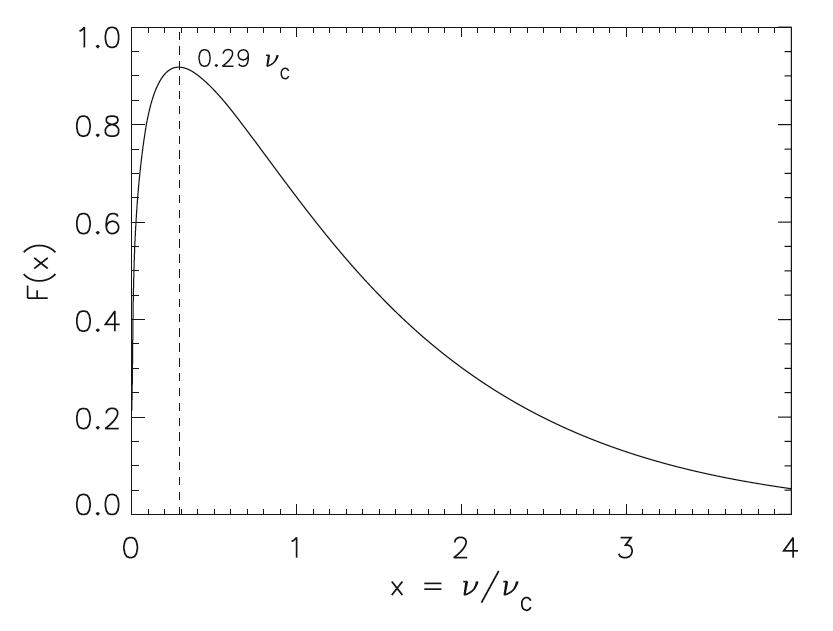
\includegraphics[width=0.8\textwidth]{images/sync_spectrum.png} 
\caption[]{Synchrotron spectrum of a single particle from \citet{Beckmann12}. The total power $F(x)$ is in unit $x=\nu/\nu_g$. }
\label{fig:sunc_spectrum}
\end{figure}

\subsection{Synchrotron emission of a particle plasma}

Up until now only the synchrotron emission of a single particle in a magnetic field has been studied.
In astrophysical sources this is unlikely to happen.
In general the observed emission is produced by a large number of particles at the same time.

In order to compute the spectrum of an electron plasma it is possible to assume that the energy is all emitted at the critical frequency $\nu_c$. 
This is possible because the spectrum of a single particle is sharply peaked below this frequency (Fig.\,\ref{fig:sunc_spectrum}).
Therefore:
\begin{equation}
    \label{eq: new_crit_freq}
    \nu \sim \nu_c\sim \gamma^2 \nu_g = \left(\frac{E}{mc^2}\right)^2\nu_g.
\end{equation}
It is easy to see that the frequency of the emission directly depends on the energy of the electron, therefore, on the electron energy distribution.
If it is considered that the electrons have a continuum distribution of energy in the interval $E_1$--$E_2$ the total emissivity of the emission is:
\begin{equation}
    \label{eq:emiss_1}
    \epsilon(\nu) = \int_{E_1}^{E_2} L(E,\nu) n(E)dE
\end{equation}
where $n(E)dE$ is the number density of the electron in the energy interval between $E$ and $E+dE$.
The energy distribution is often a power-law, and it can be written in the following way:
\begin{equation}
    \label{eq:powerlaw}
    n(E)dE=kE^{-p}dE,
\end{equation}
where $k$ is the normalization of the power-law, $p$ is the index and they are both constant.
If $p>0$, as it typically happens in astrophysical sources, Eq.\,\ref{eq:powerlaw} means that the number of electrons decreases at higher energies.
Integrating Eq.\,\ref{eq:emiss_1} assuming the power-law in Eq.\,\ref{eq:powerlaw}, it is possible to obtain the synchrotron emissivity. 
The luminosity emitted per unit volume and unit time is:
\begin{equation}
    \label{eq:emiss_2}
    \epsilon(\nu)=\frac{\sqrt{3}e^3}{2mc^2}\left(\frac{3e}{4\pi m^3 c^5}\right)^{\frac{p-1}{2}}k\left(B\sin\beta\right)^{\frac{p+1}{2}}\nu^{\frac{1-p}{2}}G\left(\frac{\nu}{\nu_{c1}},\frac{\nu}{\nu_{c2}},p\right)
\end{equation}
where $\nu_{c1}$ and $\nu_{c2}$ are the critical frequencies at energies $E_1$ and $E_2$, while $G\left(\frac{\nu}{\nu_{c1}},\frac{\nu}{\nu_{c2}},p\right)$ is a function that is reduced to:
\begin{equation}
    \label{eq:G}
    G\left(0,\infty,p\right) = \frac{2^{\frac{p-3}{2}}}{3}\left(\frac{3p+7}{p+1}\right)\Gamma\left(\frac{3p-1}{12}\right)\Gamma\left(\frac{3p+7}{12}\right),
\end{equation}
where $\Gamma$ is the gamma function, when $\nu_{c1}\ll\nu\ll\nu_{c2}$.
Eq.\,\ref{eq:emiss_2} does not depend on $\nu$, therefore:
\begin{equation}
    \label{eq:emiss_3}
    \epsilon(\nu) \propto \nu^{\frac{1-p}{2}}.
\end{equation}
Usually the quantity $\alpha_R = \frac{p-1}{2}$ is called radio spectral index.
The slope of the radio spectrum is directly connected to the slope of the electron energy distribution.
In the case of some of the brightest radio sources in the Universe, flat spectrum radio quasars (FSRQ), the radio continuum has a spectral index $\alpha_R \sim 0.5$, produced by an electron energy distribution $n(E)\propto E^{-2}$.
The spectrum can have a high frequency cut-off that depends on the critical frequency of the most energetic electrons.

\section{Thermal emission}
\label{sec:thermal_emission}

\blfootnote{This section is partially extracted from \citet{Robson} and \citet{Beckmann12}.}
Synchrotron emission is probably the dominant continuum emission process in a large part of the AGN SED, in particular at low frequencies.
However, in the IR-optical-UV range the continuum emission of most classes of AGN is dominated by thermal processes such as black body radiation.
In the IR band most of the emission is produced by dust via thermal emission, while in the optical and UV range some AGN show an excess of emission with respect to the underlying power law produced by the synchrotron process, the so called \emph{big blue bump}.

The big blue bump is particularly interesting for two main reasons: its high energy UV radiation is important for the ionization of the gas and it has often been associated with thermal radiation from the accretion disk of the AGN.

For this reason, even though thermal processes are usually associated with stars more than with AGN, the following section will summarize the main characteristics of some thermal emission processes.

\subsection{Black body radiation}


\begin{figure}
\centering
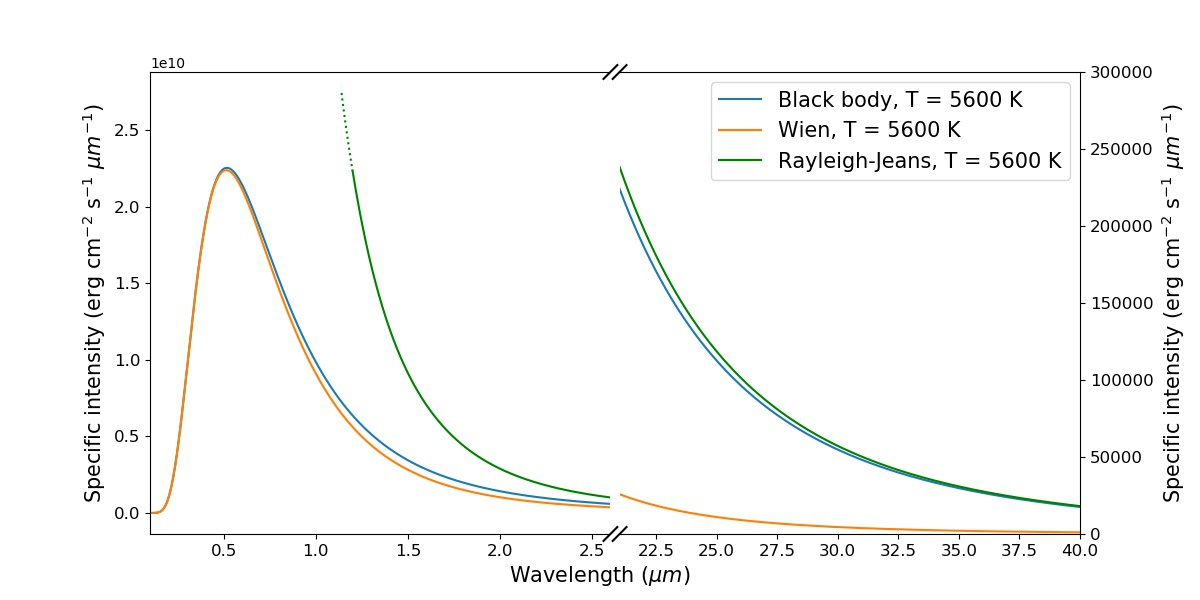
\includegraphics[width=0.8\textwidth]{images/BB.jpg} 
\caption[]{Black body spectrum and traditional approximations at high and low energies. The blue line represent the black body emission at a temperature $\rm T = 5600\,\si{K}$. The green line is the Rayleigh-Jeans approximation for $h\nu/kT<<1$, while the orange line is the Wien approximation for $h\nu/kT>>1$. Both approximation are measured for $\rm T = 5600\,\si{K}$. The left panel shows the high energy end of the spectrum, while the right panel is a zoom in on the low energy tail, where the Rayleigh-Jeans approximation  is valid.}
\label{fig:BB_emission}
\end{figure}

Black body emitters are probably the most common emitters of the whole Universe.
A black body is a body in thermal equilibrium with its surroundings and it is a perfect absorber, and emitter, of radiation.
The emission of a black body is isotropic and it is not polarized.
A black body is a theoretical construct and it is almost impossible to build in laboratory.
However, stars are a reasonable approximation of black bodies and they can be treated in this way for most common applications.

The main property of a black body radiator is its peculiar spectrum which depends only on the temperature of the black body and on none of its other properties.
The shape of the spectrum is well described by the so called \emph{Planck's law}:
\begin{equation}
    \label{eq:planck}
    B_{\nu}(T) = \frac{2h\nu^3}{c^2}\frac{1}{\exp{\left(\frac{h\nu}{kT}\right)} - 1},
\end{equation}
where $h$ is the Planck constant, $c$ is the speed of light, $k$ is the Boltzmann constant and $T$ is the temperature of the black body.
In Eq.\,\ref{eq:planck}, $B_{\nu}(T)$ is expressed as a function of the frequency, but it is easy to write the Planck's law as a function of wavelengths considering that:
\begin{equation}
    \label{eq:transform}
    B_{\nu}d\nu = B_{\lambda}d\lambda.
\end{equation}

To better understand the properties of this curve it is useful to consider two limits.
For low frequencies, where $h\nu/kT \ll 1$, the equation can be simplified to:
\begin{equation}
    \label{eq:rj}
    B_{\nu}(T) = \frac{2h\nu^2kT}{c^2}
\end{equation}
which is the so called Rayleigh-Jeans approximation.
Eq.\,\ref{eq:rj} says that all black bodies at low frequencies can be approximated by a power law with index $\alpha = 2$.
On the other extreme of the frequency range, for $h\nu/kT \gg 1$, the Wien approximation applies:
\begin{equation}
    \label{eq:wien}
    B_{\nu}(T) = \frac{2h\nu^3}{c^2}\exp\left(-\frac{h\nu}{kT}\right)
\end{equation}
which says that the spectrum drops rapidly with an exponential cutoff.
Fig.\,\ref{fig:BB_emission} shows the spectrum of a black body with a temperature of $\rm T=5600\,\si{K}$ and the two above mentioned approximations.

From the two approximations it is clear that when $h\nu/kT \sim 1$ the black body spectrum has a maximum and it is possible to prove that this peaks depends only on the temperature of the body.
In particular the relation is:
\begin{equation}
    \label{eq:wien_disp}
    \lambda_{max}T=K,
\end{equation}
where $K$ is a constant.
Eq.\,\ref{eq:wien_disp} is called Wien Displacement Law.
This is a really useful relation because it can be used to estimate the temperature of a black body (e.g. a star) from a relatively easy measure of the wavelength of its peak.

The last fundamental property of the black body radiation is its Luminosity.
Integrating Eq.\,\ref{eq:planck} over the frequency it is possible to obtain the energy flux radiated by a black body:
\begin{equation}
    \label{eq:stef-boltz}
    F = \sigma T^4.
\end{equation}
This equation is called Stefan-Boltzmann law and confirm that most of the properties of the black body emission are related to the temperature of the black body itself.
It is easy to calculate the radiated luminosity of the black body from Eq.\,\ref{eq:stef-boltz}:
\begin{equation}
    \label{eq:luminosity}
    L = 4\pi r^2 F = 4\pi r^2\sigma T^4,
\end{equation}
which depends only on the dimension of the source and on its temperature.
Luminous objects can either be hot, large or both.

\section{Free-free emission}

\begin{figure}
\centering
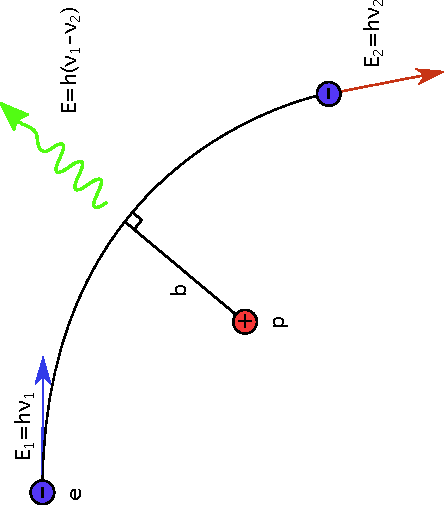
\includegraphics[width=0.6\textwidth, angle =270]{images/free_free.pdf} 
\caption[]{Scheme of the production of free free radiation by an electron with energy $E_1 = h\nu_1$ interacting with a stationary proton. After the interaction the electron goes away with an energy $E_2=h\nu_2$ after emitting a photon with an energy $E=h(\nu_1-\nu2)$.}
\label{fig:free_free}
\end{figure}

Free-free emission, also called \emph{thermal bremsstrahlung} from the German word for ``braking radiation'', is the continuum radiation emitted by charged particle (usually electrons) scattered by an ion.
During this process, a charged particle interacts with an ion and as a consequence of the interaction it changes its path, it is accelerated, emitting radiation (Fig.\,\ref{fig:free_free}).
The name free-free radiation comes from the fact that the charged particle move from a free state to another free state with lower energy and it is not bound to the ion in any moment of the process.
Free-free radiation is typical of hot plasma in non relativistic conditions.

To describe this emission process an ion with charge $Ze$ and a free electron will be considered.
Since the mass of the ion is always several orders of magnitude larger with respect to the mass of the electron, it is possible to consider the ion being at rest in every moment of the scattering, and the electron the only particle accelerated in the process.
Considering the electron at a distance $d$ from the ion, with $d$ changing with time with the electron motion, the acceleration felt by the electron is:
\begin{equation}
    \label{eq:acceleration}
    a = \frac{F}{m} = \frac{Ze^2}{md^2}\approx \frac{Ze^2}{mb^2},
\end{equation}
where it has been considered that the majority of the acceleration is produced when the electron is at the minimum distance $b$ form the ion.
This value $b$ is called the impact parameter.
It is possible to calculate the luminosity emitted as a function of the distance \citep{Deyoung02}:
\begin{equation}
    \label{eq:free_lum}
    L(d) = \frac{2Z^2e^6}{3c^3m^2d^4}.
\end{equation}
$L(d)$ strongly depends on the distance with $d^{-4}$, therefore the most of the emission is produced when the electron is close to the ion, at a distance $d<\sqrt{2}b$.
Moreover, the longer the electron stays close to the ion, the more it is accelerated.
The time that the electron spend close to the ion is easy to calculate in the non relativistic case and it is simply $\Delta t = 2b/v$, where $v$ is the relative velocity of the electron with respect to the ion.
It is possible to use this last equation with Eq.\,\ref{eq:free_lum} to derive the energy released by a single electron during the scattering:
\begin{equation}
    \label{eq:free_energy}
    E(b,v) = \frac{4Z^2e^6}{3c^3m^2b^3v},
\end{equation}
where it has been considered that most of the energy is produced when $d\sim b$.
The maximum of the energy is produced also at a peculiar frequency, which is related to the time $\Delta t$.
This frequency can be expressed as $\omega_{max} = \pi/\Delta t = \pi v/2b$ and it can be used to recover the energy emitted per unit frequency:
\begin{equation}
    \label{eq:free_energy_freq}
    E(b,v) = \frac{8Z^2e^6}{3\pi c^3m^2b^2v^2}.
\end{equation}

Once calculated the emission of a single electron, it is possible to calculate the emission of the whole plasma which will depend on the number of scattering events per unit time $N = n_i \sigma v$, where $n_i$ is the ion density and $\sigma = \int 2\pi b db$ is the cross section for the scattering.
Not all the impact parameter $b$ will produce a significant amount of emission, but only those for which the electron is close enough, $b\lesssim v/\omega$. 
It is also convenient to assume that the change in direction of the electron is small, in order to have $\Delta v \lesssim v$.
Such conditions allow to obtain some $b_{min}$ and $b_{max}$ and, assuming an electron density $n_e$ it is possible to measure the emissivity
\begin{equation}
    \label{eq:free_emissivity} 
    \epsilon(v) = \frac{16 Z^2 e^6 n_e n_i}{3c^3m^2v}\ln\frac{b_{max}}{b_{min}}.
\end{equation}
The quantity $\epsilon(v)$ is clearly a function of velocity, therefore to obtain the total emissivity of the plasma a velocity distribution must be assumed.
In most astrophysical cases, free-free emission is produced in plasma where the electron velocity distribution can be described by a Maxwell-Boltzmann distribution, and this is why free-free emission is usually considered a thermal emission.
Integrating Eq.\,\ref{eq:free_emissivity} considering this velocity distribution and a minimum and maximum velocity of the particles, it is possible to obtain:
\begin{equation}
    \label{eq:free_emissivity_total}
    \epsilon(v) = \frac{16 Z^2 e^6 n_e n_i}{3c^3m^2}\bar{g}_{ff}\frac{4\pi^2}{\sqrt 3}(2\pi)^{-3/2}\sqrt{\frac{m}{kT}} \exp\left(\frac{-mv^2_{min}}{2kT}\right).
\end{equation}
The new parameter $\bar{g}_{ff}$ is called Gaunt factor and it is a quantum mechanical correction of the $\ln(b_{max}/b_{min})$ expression.
For the integration it has been considered that $v_{max} = \infty$ while $v_{min}$ must be large enough that $\frac{1}{2}mv^2 = h\nu$ in order to produce the photon.
Finally, the total luminosity per unit volume is:
\begin{equation}
    \label{eq:free_lum_tot}
    L=\frac{32 \pi Z^2 e^6}{3c^3m^2}\bar{g}_{\nu}\sqrt{\frac{2 \pi m k T}{3h^2}}n_e n_i.
\end{equation}
The luminosity is proportional to the density of the plasma and it also increases with $\sqrt T$.
The free-free emission is an efficient cooling process.

\clearpage 
\section{Emission lines}
\label{sec:emission_line}

\blfootnote{This section is partially extracted from \citet{Barbieri91}, \citet{Dopita03}, \citet{OsterbrockAGN} and \citet{LaMuraSpec}.}
Optical AGN spectra are often characterized by strong emission lines which are emitted by several different atoms or ions.
Such lines are fundamental to study the properties of the gas in the different AGN structures.
The identification of the lines and the measurement of their observed wavelengths is an easy way to estimate the redshift of the AGN, the width of the line and its general profile is a proxy of the gas internal motion, and their relative strength is fundamental to investigate the physical condition of the emitting gas.

Each emission line corresponds to the transition of an electron between two energy levels in the same atom.
These transition are governed by the law of quantum mechanics and they usually must satisfy what are called the selection rules for electric dipole emission:
\begin{itemize}
    \item $\Delta S = 0$
    \item $\Delta L = 0,\pm1$ and $L =0 \not\to L=0$
    \item $\Delta J = 0, \pm 1$ and $J=0 \not\to J=0$
    \item $\Delta l = \pm 1$
\end{itemize}
where $S$ is the total spin quantum number, $L$ is the orbital quantum number, $J$ is the total angular momentum quantum number and finally $l$ is the orbital quantum number of the single electron. 

In an atom, the only electron that can move between levels is one of those in the outermost incomplete shell. 
These valence electrons spend most of their time in the level with the minimum possible energy allowed by the Pauli exclusion principle\footnote{The Pauli exclusion principle says that no fermions can exist in an atom with exactly the same quantum numbers.}.
When the electrons are in this level, it is said that the atom is in the ground state, while when one of them is on a higher energy level the atom is in an excited state.
In order to emit a photon, the atom must be in an excited state and the transition must be towards the ground state or to another excited state with a lower energy.

The strength of a transition between two levels (let us call them level 1 and level 2) is determined by the probability that an excited atom will emit a photon per unit time in that transition.
This transition probability is also called \emph{Einstein coefficient for spontaneous emission} $A_{21}$ and it is defined by the following relation:
\begin{equation}
    \label{eq:einstein1}
    A_{21} = \frac{64\pi^{4}\nu_{12}^3}{3hc^3g_2}S_{21}
\end{equation}
where $S_{21}$ is the so called \emph{line strength} and $g_2$ is the statistical weight of the level 2, $g_i = 2J_i+1$.
$A_{21}$ is measured in s$^{-1}$ and it is the inverse of the mean time that an electron spend on level 2 before moving to level 1 emitting a photon.
From Eq.\,\ref{eq:einstein1} it is possible to see that the transition probability is strongly dependent on the frequency of the transition itself, so if there are multiple possible transitions for the electron the one with the highest frequency (or the shortest wavelength) is preferred.
The transitions respecting the selection rules usually have high probabilities, $A_{21}\sim 10^8$--$10^9\,\si{s^{-1}}$ and they are called \emph{permitted transitions}.

As it has been previously said, to emit a photon, the atom must be in an excited state.
One of the possible mechanisms to excite an atom is the photoexcitation.
When an atom is placed in an electromagnetic field with energy density $U(\nu_{12})$, where $\nu_{12}$ is the frequency of the transition, there is a probability for the atom to absorb one photon and jump to an excited state.
This transition probability is defined as $B_{12}U(\nu_{12})$ where $B(\nu_{12})$ is called \emph{Einstein coefficient for absorption}.
However, in the same situation, an atom can also be deexcited into a lower level with a probability $B_{21}U(\nu_{12})$ emitting a photon which is a copy of the incoming one.
This process is called stimulated emission and $B_{21}$ is the \emph{Einstein coefficient for stimulated emission}.
$B_{21}$ is defined by:
\begin{equation}
    \label{eq:einstein2}
    A_{21} = \frac{8\pi h\nu_{21}^3}{c^3} B_{21}.
\end{equation}
$B_{12}$ and $B_{21}$ are linked by the following relation:
\begin{equation}
    \label{eq:einstein3}
    g_2B_{21} = g_1B_{12}.
\end{equation}
This equations means that absorption and stimulated emission are competing between each other, and that the relative importance of the first with respect to the other depends on the amount of atom in level 2 and level 1.
In usual astrophysical conditions the dominant process is absorption, stimulated emission become dominant only in peculiar cases such as in masers. 

The concept of permitted transitions has already been introduced.
But if there are permitted transition there should be also \emph{forbidden transitions}.
These are all the observed transitions where the electron should not be allowed to perform the jump, according to the electric dipole selection laws.
However, in astrophysical optical spectra it is possible to observe multiple lines which cannot be related to permitted transition and that must be the result of an electron deexciting through a forbidden transition.
In AGN in particular these often are the strongest lines and they typically are associated to elements heavier than He.
On the other hand, typical permitted lines observed in these objects are \emph{recombination lines} such as those of the hydrogen Balmer series.

In the following section the properties of recombination lines and of forbidden lines and their importance in active galactic nuclei will be shortly described.

\subsection{Recombination lines}

The easiest atom to look for when describing spectroscopic transitions are those ions where 
there is a single electron orbiting around a nucleus of charge Z.
Since this is the situation always happening in an hydrogen atom, where a single electron is bounded to a single proton, this class of ions is called \emph{Hydrogenic ions}.
For simplicity the hydrogen atom will be considered in the following discussion.

In the low density limit, the vast majority of the lines produced by hydrogen is the consequence of a recombination process, when a free electron get captured by a nucleus (typically a free proton).
Other processes such as stimulated emission and ionization or excitation from excited states are negligible.
The recombination can happen only in two ways: 
\begin{itemize}
    \item a direct recombination to the ground level,
    \item a recombination to an excited level followed by a transition cascade to the ground state.
\end{itemize}
From observations it is clear that the emitting gas is in statistical equilibrium because the emission lines do not rapidly change as expected in the opposite case.
Statistical equilibrium means that the populations of the levels are constant, and therefore for each leaving electron there should be another electron which arrives to populate the level:
\begin{equation}
    \label{eq:statistical_eq}
    N_n\sum\limits_{m=1}^{n-1} A_{nm} = \sum\limits_{m=n+1}^{\infty} A_{mn}N_m + N_pN_e\alpha_{0n}(T_e).
\end{equation}
The left part of the equation represents the electrons leaving the level downward, where $N_n$ is the number density of atoms in the level $n$ and $A_{nm}$ is the Einstein coefficient for spontaneous emission.
The right part represents the electrons arriving to level $n$. 
The first term is the number of electron arriving from upper levels via photon emission, with the same meaning of the symbols as in the left part of the equation, while the second term is the number of electron directly recombining to level n.
Here $N_p$ and $N_e$ are the densities of protons and electrons respectively (the hydrogen case has been considered here) and $\alpha_{0n}(T_e)$ is the coefficient of direct recombination to level $n$ as a function of electron temperature $T_e$\footnote{The electron temperature is defined as the temperature of the Maxwell-Boltzmann distribution used to describe the velocity distribution of the electrons}.

In thermodynamic equilibrium, which happens when every energy exchange process is perfectly balanced by its own inverse, it is possible to use the Saha equation to describe the ionization state of the gas and the Boltzmann equation to describe the population of the levels:
\begin{gather}
    \label{eq:saha}
    \frac{N_pN_e}{N_1} = \left(\frac{2\pi m_e k T}{h^2}\right)^{3/2}\exp(-h\nu_0/kT)\\
    \label{eq:bolt}
    \frac{N_n}{N_1} = \frac{2n^2}{2} \exp(-\chi_n/kT)
\end{gather}
where $m_e$ is the electron mass, $k$ is the Boltzmann constant, $h$ is the planck constant and $\chi_n$ is the excitation energy of the level n with respect to the ground state.

Combining the previous equation it is possible to obtain the density of atoms in the level $n$ as:
\begin{equation}
    \label{eq:number_density}
    N_n = N_pN_en^2\left(\frac{h^2}{2\pi m_e k T}\right)^{3/2} \exp\left(-\frac{h\nu_0 -\chi_n}{kT}\right)
\end{equation}
In general the thermodynamic equilibrium cannot be assumed, but the results is still valid if the right part of the equation is multiplied by a coefficient $b_n$ called the departure coefficient from the thermodynamic equilibrium. It is possible to substitute Eq.\,\ref{eq:number_density} in Eq.\,\ref{eq:statistical_eq} obtaining:

\begin{multline}
    \label{eq:statistical_eq2}
    b_n \sum\limits_{m=1}^{n-1} A_{nm} = \sum\limits_{m=n+1}^{\infty} \frac{m^2}{n^2}b_m A_{mn} \exp\left(\frac{\chi_m-\chi_n}{kT}\right) \\
    + \alpha_{0n}(T_e)\left(\frac{2\pi m_e kT}{h^2}\right)^{3/2}\exp\left(-\frac{h\nu_0 - \chi_n}{kT}\right)
\end{multline}

Solving this equation is not trivial, but it allows to find the values for the $b_i$ coefficient for each level.
Once $b_i$ is known, it is possible to use Eq.\,\ref{eq:number_density} to find the population of the level $n$ and therefore the intensity $I^L_{\nu}$ for each line:
\begin{equation}
    \label{eq:emission_coef}
    I_{\nu}^L = F_{nm}(T_e)\int_0^{r*}N_pN_ndr,   
\end{equation}
where all the line properties are grouped in the function $F_{nm}$.

Up until now, only the so called Case A has been considered, where the gas is optically thin in all the emission lines.
However, this only happens in very diffuse nebulae which are extremely difficult to observe because of their low surface brightness.
A more realistic condition observed in nebulae, and also in AGN, is the Case B.
Case B happens when the optical depth in the Lyman series is so high that the series is optically thick.
Typical values of the optical depths for Ly$\alpha$ are around $\tau \approx 10^4$ \citep{OsterbrockAGN}, meaning that the mean free path of a Ly$\alpha$ photon is so short that it is almost immediately reabsorbed by another atom. 
This is true not only for Ly$\alpha$ but for all the Lyman lines, even though the optical depth changes with the line.
Moreover, every time that a Lyman photon with energy higher than that of Ly$\alpha$ is absorbed and emitted, there is some finite probability that the emitting transition is decomposed in 2 or more transitions emitting lower energy photons.
For example, a Ly$\beta$ photon can be decomposed in a Ly$\alpha$+H$\alpha$, a Ly$\gamma$ in a Ly$\alpha$+H$\beta$ or Ly$\alpha$+H$\alpha$+Pa$\alpha$ and so on.
In Case B therefore all the Ly$\alpha$ photons are emitted and absorbed almost instantaneously and can be ruled out from the sums of Eq.\,\ref{eq:statistical_eq2}.
Apart from this exception the equations are the same and it is possible to measure, with accurate precision, the flux of each hydrogen lines in both cases.

Hydrogen recombination lines are important in AGN because they are some of the strongest lines which can be observed from the BLR.
They are therefore fundamental to investigate the properties of the gas in this particular region.
Unfortunately they are not strongly variable as a function of temperature or density of the gas, they cannot be used to directly measure these quantities.
Moreover the gas conditions are quite different from those assumed in Case A and Case B calculations, therefore other processes beside recombination might contribute to the statistical balance and it is more difficult to have precise flux values.
However they trace the kinematics of the gas and the amount of ionizing photons, making them fundamental in the study of the BLR structure.

On the other hand, it is possible to say that the gas in the NLR can be well approximated by the Case B scenario.
Precise line ratios can be calculated and a comparison with the observed values can be used to estimate important quantities such as dust extinction.
 
\subsection{Forbidden lines}
\label{sec:forb_line}

Some of the strongest emission lines observed in optical spectra are not recombination lines but forbidden lines (e.g. [\ion{o}{III}]$\lambda5007$, [\ion{n}{ii}]$\lambda6584$, [\ion{S}{ii}]$\lambda\lambda6717,6731$)\footnote{To visually discern between permitted and forbidden lines, the name of the emitting ion in the latter is traditionally wrapped in square brackets.}.
As it was already introduced, forbidden transitions are transitions that do not follow the selection rules presented in Sec.\,\ref{sec:emission_line} for electric dipole.
However, they are allowed in another approximation, the \emph{magnetic dipole approximation}.

The main difference between permitted and forbidden lines is that the coefficient of stimulated emission of the latter is several order of magnitudes smaller with respect to that of permitted transitions.
There are two direct consequences of this:
\begin{itemize}
    \item the mean lifetime of the excited level is longer ($\Delta t \approx A_{nm}^{-1}$);
    \item the Einstein coefficient of absorption is low (Eq.\,\ref{eq:einstein2}, \ref{eq:einstein3}).
\end{itemize}
Therefore, the ion cannot be excited by photoexcitation and once it is excited via another process, the electron can stay in the excited state for times of the order of seconds or minutes before moving to another level via photon emission.

The mechanism usually involved in the excitation of these ions is \emph{collisional excitation}.
The ion is excited via collision with a charged particle, usually electrons and in some cases protons.
In this case the exchange of energy and momentum is not limited by the selection rules because the colliding particle can be used to balance the transition.
It must be considered that the collision between an ion and a particle can populate an excited level, but it can also depopulate it, if the electron stays in the excited state for a long enough time.
For this reason forbidden lines can be emitted only in a range of electron densities where the maximum density corresponds to the density where collisional deexcitation completely balance collisional excitation.
This value depends on the mean lifetime of the level, since the longer it is, the easier the excited ions can be involved in a collision before emitting a photon.

The efficiency of the collisional excitation depends on the \emph{collisional cross section}.
Considering again an atom with a ground state and a single excited state (1 and 2 respectively), the cross section is defined by:
\begin{equation}
    \label{eq:crosssection}
    \sigma_{12}(E) = \left(\frac{h^2}{8\pi m_e E}\right)\left(\frac{\Omega_{12}}{g_1}\right)
\end{equation}
where $\Omega_{12}$ is the \emph{collision strength}, a quantity that does not depend on the energy of the transition and that it is symmetric with respect to the lower and upper state, $\Omega_{12} = \Omega_{21}$.

It is possible to derive some interesting properties of forbidden lines with this two level model.
Let us consider the equilibrium between collisional excitation and radiative depopulation in the low density limit:
\begin{equation}
    \label{eq:equilibrium_forbidden}
    R_{12} = A_{21}N_2,
\end{equation} 
where $R_{21}$ is called the rate of population of the upper level per unit volume through collisional excitation:
\begin{equation}
    \label{eq:rate_population}
    R_{12} = N_eN_1 \alpha_{12}.
\end{equation}
In this equation, $\alpha$ is the collisional excitation coefficient.
Using Eq.\,\ref{eq:rate_population} in Eq.\,\ref{eq:equilibrium_forbidden} and expanding $\alpha_{12}$ the equilibrium equation became:
\begin{equation}
    \label{eq:equilibrium_forbidden2}
    N_2 = N_e N_1 \beta A_{21}^{-1}T^{-1/2}\left(\frac{\Omega_{12}}{g_1}\right)\exp\left(\frac{-E_{12}}{kT}\right),
\end{equation}
where $\beta = [(2\pi \hbar^4)/(km_e^3)]^{1/2}$ is a constant.
The flux of the emission line is just the product of the number of transition per unit of time and the energy of each photon:
\begin{equation}
    \label{eq:flux}
    F_{12} = \chi_1 N_e^2 \beta E_{12} T^{-1/2} \left(\frac{\Omega_{12}}{g_1}\right) \exp\left(\frac{-E_{12}}{kT}\right).
\end{equation}
In this equation $N_1 = \chi_1N_e$ with $\chi_1$ the number fraction of the ion at level 1.
This equation is important because it shows the dependence of the flux of the line from the gas temperature.
At low temperature the line rapidly fades because the exponential is the dominant term, while at high temperature $T^{-1/2}$ dominates and the line slowly fades.
In the high density limit, the level population are set by the Boltzmann equation and the flux of the line is:
\begin{equation}
    \label{eq:flux_boltz}
    F_{12} = \chi_1 N_e E_{12} A_{21} \left(\frac{g_2}{g_1}\right) \exp\left(\frac{-E_{12}}{kT}\right).
\end{equation}
The dependence on the electron density $N_e$ changes from $N_e^2$ to $N_e$, which implies that a \emph{critical density} $n_c$ exists. 
$n_c$ represent the density where the collisional and radiative depopulation equally contribute to the depopulation of the excited level,  $A_{21} N_2 = R_{21}$.
$R_{21}$ is the rate of depopulation through collisional deexcitation.
After some calculation results that:
\begin{equation}
    \label{eq:critic_dens}
    n_c = \frac{A_{21}g_2T^{1/2}}{\beta\Omega_{12}}.
\end{equation}
From Eq.\,\ref{eq:critic_dens} it is possible to see that $n_c$ depends on $A_{12}$ and $\Omega_{12}$ and therefore each transition has a different critical density.
The presence or the absence of a peculiar emission line can therefore be used to roughly estimate the electron density of an astrophysical gas.
The best example is the case of the BLR of an AGN. 
No broad forbidden line are seen in the spectra of this region, meaning that the density is significantly higher with respect to the highest critical density, i.e. [\ion{o}{iii}]$\lambda5007$ \citep[$n_c \approx10^6\,\si{cm^{-3}}$][]{OsterbrockAGN}.
In the high density regime the line fades as $n_c/n_e$, therefore the density should be at least higher than $10^8\,\si{cm^{-3}}$ to completely avoid level depopulation via photon emission.
There are not forbidden line that can be used to estimate an upper limit, but in the UV range is it possible to observe a broad \ion{c}{III}]$\lambda1909$ line, which arises from a semi-forbidden transition\footnote{Semi-forbidden transition are transitions that are possible only in the electric quadrupole approximation.}.
Also semi-forbidden lines have a critical densities and $n_c\approx 10^{10}\,\si{cm^{-3}}$ for \ion{c}{III}]$\lambda1909$, meaning that the density of the BLR gas should be between $10^8$ and $10^{10}\,\si{cm^{-3}}$.

\paragraph{Tree-level atom}

\begin{figure}
\centering
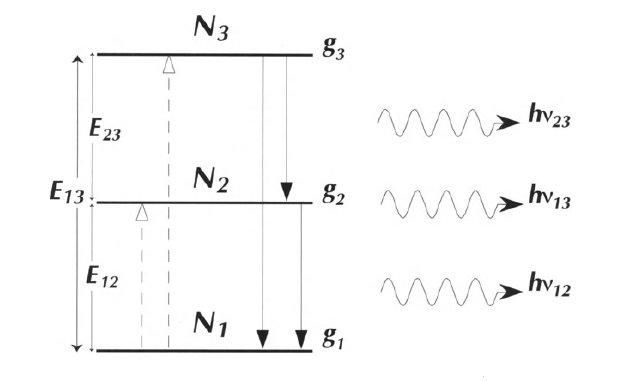
\includegraphics[width=0.8\textwidth]{images/o3_scheme.png} 
\caption[]{Three level system in the low density limit, e.g. [\ion{O}{III}] \citep{Dopita03}.  }
\label{fig:o3_scheme}
\end{figure}

Even though the two levels model can be useful to derive some properties of forbidden lines, the physics of most of the observed lines can be better described by the three-level atom.
The levels involved in the transitions often have the same principal quantum number, but they have been split in energy by quantum mechanic effects such as spin-orbit interaction, which are not described here.

The population of the levels can be recovered considering the equations of the statistical equilibrium:
\begin{align}
    \label{eq:threelevel_equilibrium}
    N_1 C_{13}+N_2 C_{23} &= N_3(C_{31}+C_{32}+A_{32}+A_{31}), \notag\\
    N_1 C_{12}+N_3(C_{32}+A_{32}) &= N_2(C_{23}+C_{21}+A_{21}),\\
    N_1+N_2+N_3 &= 1. \notag
\end{align}
While the $A_{nm}$ coefficients are the usual spontaneous emission coefficients, the terms $C_{nm}$ are called collision rates.
If $n>m$ the rate represents collisional deexcitation, vice versa it represents collisional excitation.
In the first two equations of Eq.\,\ref{eq:threelevel_equilibrium}, the left part represents the number of electrons arriving to the level $n$, the right part the electron leaving.
The last equation is just a normalization, which says that the number densities of ions in a certain levels are expressed as a fraction of the total ion density.
This system of equations can be solved in all cases if the $C_{nm}$ and $A_{nm}$ coefficients are known, but it is useful to consider only two approximations: the low density limit (collisional deexcitation coefficients negligible) and the limit where the energy difference between the upper two levels is negligible with respect to the difference between the ground level and the excited ones.

In the simple low density limit (Fig.\,\ref{fig:o3_scheme}), the collisional deexcitation coefficients are negligible, as anticipated.
Moreover it is possible to assume two more simplifications.
First, the upper level can be collisionally excited only from the ground level, because the mean lifetime of the middle level is too short for the ion to be further involved in a collision.
Second, the number of electrons moving from the upper level to the middle one via photon emission is negligible with respect to the collisional excitation of the level, because the emission coefficient is small and it depends on $\nu^3$ (Eq.\,\ref{eq:einstein2}).
The equations now are:
\begin{align}
    \label{eq:lowdensity_equilibrium}
    N_1 C_{13} &= N_3(A_{32}+A_{31}), \notag\\
    N_1 C_{12} &= N_2A_{21},\\
    N_1+N_2+N_3 &= 1, \notag
\end{align}
and it is easy to derive $N_3 = N_1C_{13}/(A_{32}+A_{31})$ and $N_2= N_1C_{12}/A_{21}$.
Recalling that the flux of the line is just the energy of the line times the number of transitions per unit time, it is possible to recover the flux ratio between the two lines:
\begin{align}
    \label{eq:flux_forbidden1}
    \frac{F_{32}}{F_{21}} &= \frac{E_{32}}{E_{21}}\frac{A_{32}C_{13}}{(A_{32}+A_{31})C_{12}}\\
    & = \frac{E_{32}}{E_{21}}\frac{A_{32}\Omega_{13}}{(A_{32}+A_{31})\Omega_{12}}\exp \left(\frac{-E_{23}}{kT}\right) \notag
\end{align}
where the collisional rate has been expressed as a function of the collision strength, and $E_{nm}$ is the energy difference between level $n$ and $m$.
The line ratio is clearly dependent on the temperature, and this is the reason why the ratio between lines rising from this combination of levels can be used to measure the temperature of the gas.

Common ions that have transitions approximated by this model are [\ion{o}{III}], [\ion{O}{I}], [\ion{n}{ii}].
Even though in this real ions the ground level is splitted in a triplet, the splitting is so small that it is possible to use the three level approximation.
Unfortunately, the line arising from the $3\to2$ transition in these system is usually faint and it can be observed only in very high quality spectra.

\begin{figure}
\centering
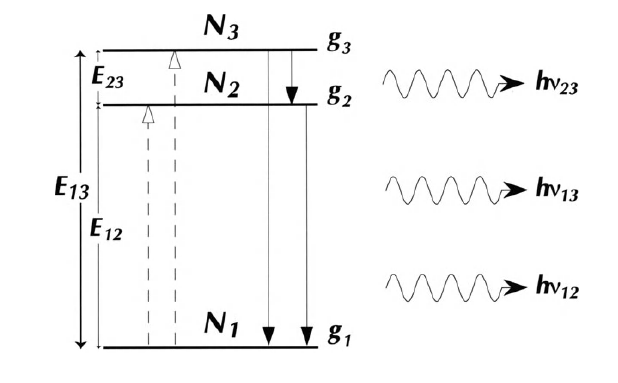
\includegraphics[width=0.8\textwidth]{images/s2_scheme.png} 
\caption[]{Three level system in the $E_{32}\ll E_{21}$ approximation, e.g. [\ion{S}{II}] \citep{Dopita03}.  }
\label{fig:s2_scheme}
\end{figure}

The second approximation assumes that $E_{32}\ll E_{21}$ (Fig.\,\ref{fig:s2_scheme}).
In this case it is possible to neglect radiative transitions between the upper levels and the system in Eq.\,\ref{eq:lowdensity_equilibrium}, considering a low density, becomes:
\begin{align}
    \label{eq:lowdensity_equilibrium1}
    N_1 C_{13} &= N_3A_{31}, \notag\\
    N_1 C_{12} &= N_2A_{21}\\
    N_1+N_2+N_3 &= 1. \notag
\end{align}
If $A_{32}$ can be neglected, also Eq.\,\ref{eq:flux_forbidden1} can be simplified:
\begin{equation}
    \label{eq:flux_forbidden2}
    \frac{F_{31}}{F_{21}} = \frac{E_{31}A_{32}N_3}{E_{21}A_{31}N_2} = \frac{E_{31}C_{13}}{E_{21}C_{12}}\sim\frac{\Omega_{13}}{\Omega_{12}}\exp \left(\frac{-E_{23}}{kT}\right)\sim\frac{\Omega_{13}}{\Omega_{12}} = \frac{g_3}{g_2}.
\end{equation}
If $E_{32}$ is negligible, the exponential can be neglected and $E_{31}\approx E_{21}$.
in the high density limit, on the other hand, the population of the level is described by the Boltzmann law, therefore $N_3/N_2 = g_3/g_2$.
The flux ratio becomes:
\begin{equation}
    \label{eq:flux_forbidden3}
    \frac{F_{31}}{F_{21}} = \frac{E_{31}A_{32}N_3}{E_{21}A_{31}N_2} = \frac{A_{31}g_3}{A_{21}g_2}.
\end{equation}
Eq.\,\ref{eq:flux_forbidden2} and Eq.\,\ref{eq:flux_forbidden3} show that the line ratio tends to a limit both at low and high density and that the two limits are different.
Moreover the limits do not depends on temperature, therefore it is possible to use the ratio between the two lines as a proxy of the gas electron density.
Typical lines used to this aim are [\ion{o}{ii}]$\lambda\lambda3726,3729$ and [\ion{S}{ii}]$\lambda\lambda6716,6731$.

\section{Shocks}
\label{sec:shocks}

\blfootnote{This section is extracted from \citet{Dopita03} and \citet{OsterbrockAGN}.}
Shocks are a peculiar emission mechanism and they are not as evident in the spectrum of AGN as the other mechanisms previously described.
However, their presence is a well established property of AGN \citep[e.g.][]{Dopita95}
and they are used to explain a wide variety of situations, starting from emission line ratios \citep[e.g.][]{Dopita95b,Dopita00,Contini02,Congiu17}, to jet knots and polarization \citep[e.g.][]{Lister05, Beckmann12}.
Shocks are also one of the main ways for the AGN to interact with its own host galaxy, since a jet expanding in the ISM produces shocks \citep{Dopita00,Fragile17}.

Shocks is able to both ionize the ISM during its passage, but radiative shocks also produce a large amounts of radiation which contribute to the photo-ionization of the gas.
A shock can be considered as a sharp discontinuity in some of the properties of the gas, in particular $\rho$, $P$ and $v$, density, pressure and velocity.
It is convenient to use a reference system moving with the shock front.
The shock motion is usually steady, therefore the reference system is moving at a constant speed.
It is also possible to describe the motion as a one-dimensional flow with the velocity components perpendicular to the shock front, and the quantity ahead and behind the shocks will be identified with the numbers 0 and 1 respectively.
In these conditions, in every instant the conservation of mass and momentum across the shock front applies and it is possible to write:
\begin{align}
    \label{eq:mass_cons}
    P_0 + \rho_0 v_0 &= P_1+\rho_1 v_1,\\
    \label{eq:momentum_cons}
    \rho_0 v_0 &= \rho_1 v_1.
\end{align}
In most conditions it is also possible to assume an adiabatic compression of the gas, therefore the equation of state become $P = K \rho^{\gamma}$ and it can be used to recover a third equation:
\begin{equation}
    \label{eq:hugoniot_3}
    \frac{v^2_0}{2} + \frac{\gamma}{\gamma-1}\frac{P_0}{\rho_0} = \frac{v^2_1}{2} + \frac{\gamma}{\gamma-1}\frac{P_1}{\rho_1}.
\end{equation}
$\gamma$ is the adiabatic index of the gas, and in most astrophysical cases, where the gas is mostly monoatomic hydrogen, its value is $5/3$.
Equation \ref{eq:mass_cons}, \ref{eq:momentum_cons} and \ref{eq:hugoniot_3} are the so called Rankine-Hugoniot conditions at the shock front and they relate the condition of the gas ahead and behind the shock.
To solve the equations it is usually assumed that the quantity ahead the shock ($\rho_0$ and $P_0$) are known and the ratios $\rho_1/\rho_0$ and $P_1/P_0$ are derived as a function of the Mach number of the shock front.
The Mach number $M$ is defined as:
\begin{equation}
    \label{eq:mach}
    M = \frac{\abs{v_0}}{c_0}
\end{equation}
where $c_0$ is the sound speed in the undisturbed gas:
\begin{equation}
    \label{eq:soundspeed}
    c_0 = \sqrt\frac{\gamma P_0}{\rho_0}.
\end{equation}

The Mach number therefore is the ratio between the velocity of the gas and the speed of sound.
The interesting limits for this number are 2: if $M\to 1$ the shock is considered a weak shock, a small disturbance in the gas propagating at the speed of sound; if $M\to\infty$ the shock is a strong shock propagating at supersonic speed.
From the previous equation it is possible to calculate the ratio of densities and pressures behind and ahead the shocks:
\begin{align}
    \label{eq:ratios1}
    \frac{P_1}{P_0} & = \frac{2\gamma}{\gamma+1}M^2 -\frac{\gamma-1}{\gamma+1},\\
    \label{eq:ratios2}
    \frac{\rho_1}{\rho_0} & = \frac{(\gamma+1)M^2}{(\gamma-1)M^2+2}.
\end{align}
In the weak shock limit both ratios tends to 1, while for $M\to\infty$ the ratios of pressures tends to $\infty$, but the ratio of densities depends on the kind of shocks: $\rho_1/\rho_0 \to 4$ for an adiabatic shock, $\rho_1/\rho_0 \to \infty$ for an isothermal shock.
As a first approximation, in common astrophysical nebulae the temperature of the gas is driven by radiative processes and it is the same ahead and behind the shock, therefore the shock can often be considered isothermal.

In an actual shock the temperature just behind the shock rises significantly, but all the energy is radiated away efficiently and the gas cools rapidly, in such a way that relatively close to the front the temperature is the same of the gas ahead of the shock.

\subsection{Radiative structure of shocks}

In the previous section it has been introduced the concept of isothermal shocks in astrophysical sources.
It has also been said that there is a small region behind the shock front which is characterized by a high temperature where the gas is able to cool rapidly.
It is in this region that most of the interesting radiative processes happens.

The structure of this region depends on the velocity of the shock, and therefore on the energy transported.
Just after the shock front, the various components of the plasma relax towards equipartition of energy in the so called \emph{equipartition zone} and all the plasma components can be described by the same temperature.
Just after that there is a region called the \emph{ionization zone}, where the lowly ionized gas coming from the pre-shock region suddenly increases its ionization degree because of the high temperature. 
If the shock is fast enough, the plasma reach a status of \emph{collisional ionization equilibrium}, where collisional ionization and recombination are in equilibrium, before entering in the following zone, the \emph{cooling zone}.
In this region the gas rapidly cools, almost isobarically, and the density increases.
During the cooling the plasma emits extreme UV photons which are able to ionize hydrogen, and if it is hot enough it can also produce X-rays.
When the temperature of the gas decreases to around $10^4\,\si{K}$, the hydrogen starts to be able to absorb the incoming UV radiation.
Since the radiation is isotropic, half of it is able to cross the shock front and it can be absorbed by the pre-shock hydrogen which can be fully ionized if the velocity of the shock is higher than $120\,\si{\kms}$.
This is important because if the plasma entering the shock is already fully ionized the structure of the shock changes.

Moving downstream the shock, to the region where the UV photon have been completely absorbed, the plasma is finally able to continue cooling and recombining.
The cooling, in all its phases, happens via emission of lines or continuum.
At the beginning, where the temperature reach its highest value, the emission is mostly in the UV range.
Several permitted lines or semi-forbidden lines of abundant ions such as \ion{c}{ii}, \ion{c}{iii}, \ion{N}{v}, \ion{o}{iv} are emitted.
When the temperature cools optical lines start to become dominant.
The ions are mostly collisionally excited, so forbidden emission lines of [\ion{O}{I}], [\ion{O}{Ii}], [\ion{O}{Iii}], [\ion{s}{Ii}] dominates the spectrum, together with hydrogen Balmer lines.
In particular, the flux in the Balmer lines strongly depends on the shock velocity and their ratio can be used to estimate this quantity.







\biblio
\end{document}